\chapter{The Photoelectric Effect}\label{ch:einstein}
\chapterprecis{Albert Einstein}

\makeoddhead{myheadings}{\emph{Einstein}}{}{\thepage}
\makeevenhead{myheadings}{\thepage}{}{\emph{The Photoelectric Effect}}

\renewcommand{\theequation}{\arabic{equation}}

\section*{Remarks}

The \emph{photoelectric effect} was discovered by Heinrich Hertz in
1887. He found that a spark passed more readily across a narrow gap in
an electric circuit if the ends of the wires were being illuminated by
ultraviolet light---when the wires were not so illuminated, the gap
between them had to be reduced in order for the spark to pass. Shortly
afterwards Wilhelm Hallwachs found that if a freshly polished zinc plate
was insulated and connected to an electroscope, it would lose an initial
\emph{negative} charge while illuminated by ultraviolet light, but that
there was no effect if the initial charge was \emph{positive}. He
concluded that negatively charged particles were being emitted under the
action of the light.

In 1900 Philipp Lenard was able to show that the negatively charged
particles emitted from metals under the action of light were identical
with the ``corpuscles'' of Thomson's cathode rays---and therefore, as we
will now say, identical with \emph{electrons}. He also showed that when
a photosensitive metal was made the cathode in a cathode ray tube and
then illuminated, a measurable \emph{photoelectric current}, carried by
these emitted electrons, passed from cathode to anode. His measurements
disclosed that this current increased steadily with the intensity of the
light falling on the cathode.

Furthermore, by opposing this photoelectric current with an
oppositely-directed electric field, Lenard was able to determine the
potential difference at which the photoelectric current was reduced to
zero---that is, the potential difference at which even the most
energetic electrons emitted from the cathode were turned back just
before they reached the anode, called the \emph{stopping potential
difference,} $\Pi$. This potential difference was a measure of the
kinetic energy with which these electrons were ejected from the
cathode.\footnote{As an emitted electron moves toward the anode against
  the electric field, its energy increases, and the work done on it by
  the field is given by the product $\Delta$\emph{Ve}, the difference in its
  potential times the charge. Since this work is done at the expense of
  the particle's kinetic energy, the particle will be brought to rest
  when its initial kinetic energy equals this product. (Compare the
  similar situation in Rutherford, Chap.~\ref{ch:rutherford}, p.~\pageref{fn:rutherford_KE}, fn.~\ref{fn:rutherford_KE}.) If this happens
  \emph{just} before it hits the anode, then its final potential
  difference with respect to the cathode is practically identical to the
  \emph{measured} potential difference between the anode and cathode.
  Assuming that all the electrons carry the same charge \emph{e}, this
  measured $\Delta$\emph{V} is directly proportional to the initial kinetic
  energy of those emitted electrons.} In this way he discovered that
this maximum kinetic energy was \emph{not} dependent on the intensity of
the illuminating light but, instead, rose with the light
\emph{frequency}.

In two major respects the photoelectric effect contradicted classical
electromagnetic wave theory:

(1) The \emph{intensity} of any wave is defined as the energy delivered
by the wave to each unit area of a surface per second.\footnote{Thus,
  for example, if all the energy in light is converted to heat upon its
  striking a perfectly non-reflecting surface, then doubling the
  intensity of the light will deliver twice as much heat per second to
  each square centimeter of the surface.} Maxwell had argued that light
is an electromagnetic wave; and he had proven mathematically that if so
then the intensity of light must be directly proportional to the square
of the \emph{amplitude}\footnote{The \emph{amplitude} of an oscillating
  quantity is the peak value which that quantity attains in each cycle,
  without regard to sign.} of the oscillating electric field which
constitutes the electric component of the wave. But the force which an
electromagnetic wave applies to an electron in its path will be
\emph{eF}, where \emph{e} is the charge on the electron and \emph{F} is
the strength of the electric field (at the location of the electron) at
any instant. If then the amplitude of the electric field increases, the
force applied to the electron at each instant likewise increases. It
would seem, then, that a more intense light beam should impart greater
kinetic energy to the electrons in its path than a light beam of lesser
intensity would. \emph{But it does not.} Increasing the light intensity
has no discernible effect on the kinetic energy of the ejected
electrons; rather it increases the \emph{number} of electrons emitted
per second from the cathode.

(2) In Maxwell's theory, the \emph{frequency} of the incident light may
play an indirect role in determining the energy imparted to
electrons---for example, the light frequency might agree or disagree
with some resonances that characterize the forces binding individual
electrons to the solid. Nevertheless such a connection must be highly
variable, and it would seem that any relation between the electron
energy and light frequency would be correspondingly complicated.
\emph{But it is not.} The relation observed between electron energy and
light frequency showed no such complexity.

Not surprisingly, in the five years between Planck's work (1900) and the
Einstein paper (1905) physicists had tried to come up with another model
that did not depend on quantization, with results ranging from partial
success to catastrophic failure (see Niels Bohr's comments in 
Chapter \ref{ch:bohr}).
Nobody was inclined to take the quantum hypothesis seriously until
Einstein adopted it.

He did more than adopt it, however. He gave a very radical answer to the
question of \emph{why} microscopic bodies could only absorb and emit
light energy in units. Planck had proposed only that the hypothetical
electrons oscillating in the radiating body emit their energy not
continuously, as Maxwell's theory would require, but rather in discrete
bursts of light, each burst containing an amount of energy, \emph{hv},
proportional to the frequency of the individual oscillating electron and
thus of the emitted light as well. He did not assume that that energy,
once emitted, would continue to travel in a discontinuous distribution,
because it would have contradicted the electromagnetic wave theory of
light, a theory that had served remarkably well. Einstein's account in
the present paper, while it harmonizes with the experimental
observations on the photoelectric effect, does contradict the
electromagnetic theory:
\begin{quote}
According to the presently proposed assumption, the energy in a beam of
light \ldots\ consists of a finite number of energy quanta, localized at
points of space, which move without subdividing and which are absorbed
and emitted only as units.
\end{quote}

Note Einstein does not call his account a \emph{theory} but rather a
``heuristic'' point of view (from ``\emph{heurisko},'' I discover)---one
intended to serve as an aid to learning or discovery.


\section*{Concerning a Heuristic Point of View about the
Creation and Transformation of Light\footnote{{[}\emph{Annalen der
  Physik}, \textbf{17} (1905), 132--148. Translated by the Editors of
  \emph{Annalen der Physik}.{]}}\\
  {\large Albert Einstein}}

There is a profound formal difference between the theoretical
representations of gases and other ponderable bodies which physicists
have constructed and Maxwell's theory of electromagnetic processes in
so-called empty space. Whereas we may consider the state of a body as
being completely determined by the positions and velocities of, to be
sure, a very large but finite number of atoms and electrons, we must use
continuous spatial functions to specify the electromagnetic state of a
region, so that a finite number of parameters cannot be considered as
sufficient to describe completely the electromagnetic state of a region
of space. According to Maxwell's theory, in all cases of pure
electromagnetic phenomena, hence in the case of light, the energy must
be considered as a continuous spatial function; whereas the energy of a
ponderable body, according to the current concepts of physicists, can be
represented by a sum taken over the atoms and electrons. The energy of a
ponderable body cannot break up into arbitrarily many, arbitrarily small
parts; whereas the energy of a ray of light emitted by a point source of
light distributes itself continuously throughout an ever-increasing
volume of space according to Maxwell's theory (or, more generally,
according to any wave theory).

The wave theory, operating with continuous spatial functions, has proved
to be correct in representing purely optical phenomena and will probably
not be replaced by any other theory. One must, however, keep in mind
that the optical observations are concerned with temporal mean values
and not with instantaneous values; and it is possible, in spite of the
complete experimental verification of the theory of diffraction,
reflection, refraction, dispersion, and so on, that the theory of light
that operates with continuous spatial functions may lead to
contradictions with observations if we apply it to the phenomena of the
generation and transformation of light.

It appears to me, in fact, that the observations of ``black-body
radiation,'' photoluminescence, the generating of cathode rays {[}by{]}
ultraviolet radiation, and other groups of phenomena related to the
generation and transformation of light can be understood better on the
assumption that the energy in light is distributed discontinuously in
space. According to the presently proposed assumption, the energy in a
beam of light emanating from a point source is not distributed
continuously over larger and larger volumes of space but consists of a
finite number of energy quanta, localized at points of space, which move
without subdividing and which are absorbed and emitted only as units.

In what follows, I want to present the thinking and indicate the facts
that have led me along the present path in the hope that the point of
view associated with these ideas may prove useful to some researchers in
their investigations.\footnote{{[}What follows is section 8 of
  Einstein's paper, sections 1--7 and 9 being here omitted. The omitted
  sections treat, among other topics, black-body radiation and Planck's
  derivation of elementary energy quanta.{]}}\\
\centerline{* * *}
%
\subsection*{VIII. On the Production of Cathode Rays by Irradiating Solid Bodies}

The traditional view that the energy of light is distributed
continuously through the region illuminated runs into great difficulty
in trying to explain photoelectric phenomena, as was outlined in a
trail-blazing paper by Lenard.\footnote{{[}\emph{Annalen der Physik}, \textbf{8}
  (1902), 169--170. We gave a brief summary of Lenard's findings above.{]}}

According to the concept that the exciting radiation consists of energy
quanta with energy content $h\nu$,\footnote{\label{fn:einstein_h}{[}Here $\nu$ is the
  light frequency and $h$ is Planck's constant. Einstein actually
  writes here not $h$ but rather a quotient of three other
  constants, introduced in omitted sections of this paper. Since there
  he shows his own expression to be equal to Planck's we take the
  liberty of substituting $h$ throughout this section. However, it
  is worth noting that his more complicated expression contains
  \emph{Avogadro's number} in the denominator. In 1905 its size was very
  conjectural.{]}} the production of cathode rays by light can be
understood as follows: Quanta of energy penetrate into the surface layer
of the body; and their energy, at least in part, is transformed into
kinetic energy of electrons. The simplest explanation is that a quantum
transfers all its energy to a single electron; we shall assume that this
occurs. However, it ought not to be excluded that electrons take up only
part of the energy of light quanta. An interior electron with kinetic
energy will have lost some of this kinetic energy by the time it reaches
the surface. Besides this we must assume that each electron will have to
do some work (an amount characteristic of the body) when it leaves the
body.\footnote{{[}The necessity for an electron to do work specifically
  to leave the surface of a body can be compared to the phenomenon of
  surface tension in a fluid. The work required is called the ``work
  function''; Einstein denotes it by \emph{P} in the expression that
  follows.{]}} The electrons lying right at the surface of the body will
leave the body with the greatest velocity normal {[}i.e.\
perpendicular{]} to the surface. The kinetic energy of such electrons is

\begin{equation*}
h\nu - P.
\end{equation*}
%
If the body is charged to the positive potential $\Pi$\footnote{{[}Thus
  there is a potential \emph{difference} $\Pi$ between the body and
  the surrounding grounded conductors, which opposes the current. This
  is exactly equivalent to what Lenard did.{]}} [\,\ldots] and if $\Pi$
is {[}just{]}\footnote{{[}We here correct an omission in the
  translation.{]}} large enough to prevent a discharge of the body, then
we must have\footnote{{[}That is, $\Pi e$,
  potential difference times charge, must equal the initial kinetic
  energy of the most energetic emitted electrons which are just stopped
  by this $\Pi$ .{]}}
%
\begin{equation*}
\Pi e = h\nu - P,
\end{equation*}
%
where \emph{e} is the electric charge of the electron, or
%
\begin{equation*}
\Pi E = Nh\nu - P'
\end{equation*}
%
where $E \: \text{[}\!= Ne\text{]}$ is the charge of a gram equivalent of a
single charged ion {[}i.e., one \emph{faraday}{]} and $P'$ is the
potential of this amount of negative charge relative to the
body.\footnote{{[}The equation $\Pi e = Nh\nu - P'$ is the
  previous equation multiplied through by Avogadro's number $N$.
  Einstein does this because in 1905 physicists had much better
  measurements for the faraday $E$ than for $e$ and Einstein
  was more confident about the size of $Nh$ than about either
  $N$ or $h$ separately. He is not worried about $P'$
  since he is about to set it to zero. {]}}

If we place $E = 9.6\times 10^3$, then $\Pi\times 10^{-8}$ is the potential
in volts that the body acquires on being irradiated in a
vacuum.\footnote{{[}The \emph{faraday} equals 96,500 cou or about 9650
  abcou. With $E$ expressed in abcoulombs and $h$ in
  erg-seconds, $\Pi$ will be given in erg/abcou or \emph{abvolts}.
  Hence $\Pi\times 10^{-8}$ will express the potential in volts. See
  Appendix.{]}}

In order to see at first if the derived relationship is of the right
order of magnitude as obtained empirically we place $P' = 0$,
$\nu = 1.03\times 10^{15}$ (corresponding to the ultraviolet limit of the
solar spectrum\footnote{{[}Sunlight comprises wavelengths as small as
  $2902\times 10^{-8}$ cm, corresponding to frequencies as great as $1.03\times 10^{15}$
  cycles/sec.{]}}) and {[}$Nh = 4.01\times 10^{-3}${]}.\footnote{{[}Einstein
  actually expresses \emph{Nh} here in terms of two other constants. His
  expression does \emph{not} contain Avogadro's number, since
  multiplying through by \emph{N} removed it from the denominator of the
  three-constant expression for $h$ mentioned in fn.\ \ref{fn:einstein_h}. 
  Note that in the cgs system of 
  measurement, Planck’s constant, $h$, has the value $6.6\times 10^{-27}\ \text{erg-sec}$.{]}} We
obtain {[}$\Pi = 4.3\times 10^8$ abvolts, so that $\Pi\times 10^{-8} =
4.3${]} volts, which agrees in order of magnitude with the results of
Lenard.\footnote{{[}In the experiments mentioned above, Lenard
  had found that when the cathode is illuminated by direct sunlight,
  electrons are emitted until the cathode acquires a potential on the
  order of a few volts.{]}}

If the derived formula is correct, then {[}$\Pi${]} must be a linear
function of the frequency whose slope {[}is independent of{]} the nature
of the material being studied.\footnote{{[}That is, the energy acquired
  by the electrons will be proportional to the frequency of the exciting
  light.{]}}

Our point of view, as far as I can see, does not contradict Lenard's
observed properties of the photoelectric phenomena. If each quantum of
energy of the exciting light gives up its energy to an electron
independently of all the other quanta, then the velocity distribution of
the electrons, that is, the characteristic of the produced cathode ray,
is independent of the intensity of the exciting radiation; on the other
hand the number of electrons leaving the body, all other conditions
being the same, will depend on the intensity of the exciting 
radiation.\\
\centerline{* * *}

\section*{Experiment: The Photoelectric Effect}

\subsection{Current is directly proportional to illumination intensity.}

If light consists of a stream of discrete quanta of energy, and if each
quantum gives up all its energy to a single electron, then the number of
electrons released per second from an illuminated photocell cathode
should equal the number of energy quanta absorbed per second by the
cathode. But the number of electrons released per second is proportional
to the \emph{cathode current}, since each electron carries a determinate
charge. And the number of energy quanta absorbed per second is
proportional to the \emph{illumination intensity}; since the very
definition of that quantity is the amount of energy absorbed, per unit
time, by unit area of the illuminated surface. Thus the current produced
by the photocell should be proportional to the illumination supplied, as
Einstein states.

To investigate this effect, a photocell is connected directly to a
sensitive picoammeter as indicated in the sketch below; set the meter to
the 2 microampere ($\mu\text{A}$) range. An ordinary
illuminating lamp makes a satisfactory light source. For a rough test of
the relation between light intensity and current, observe how the
photocurrent rises and falls when the light source is moved toward and
away from the cell.

\begin{figure}[h]
  \begin{center}
  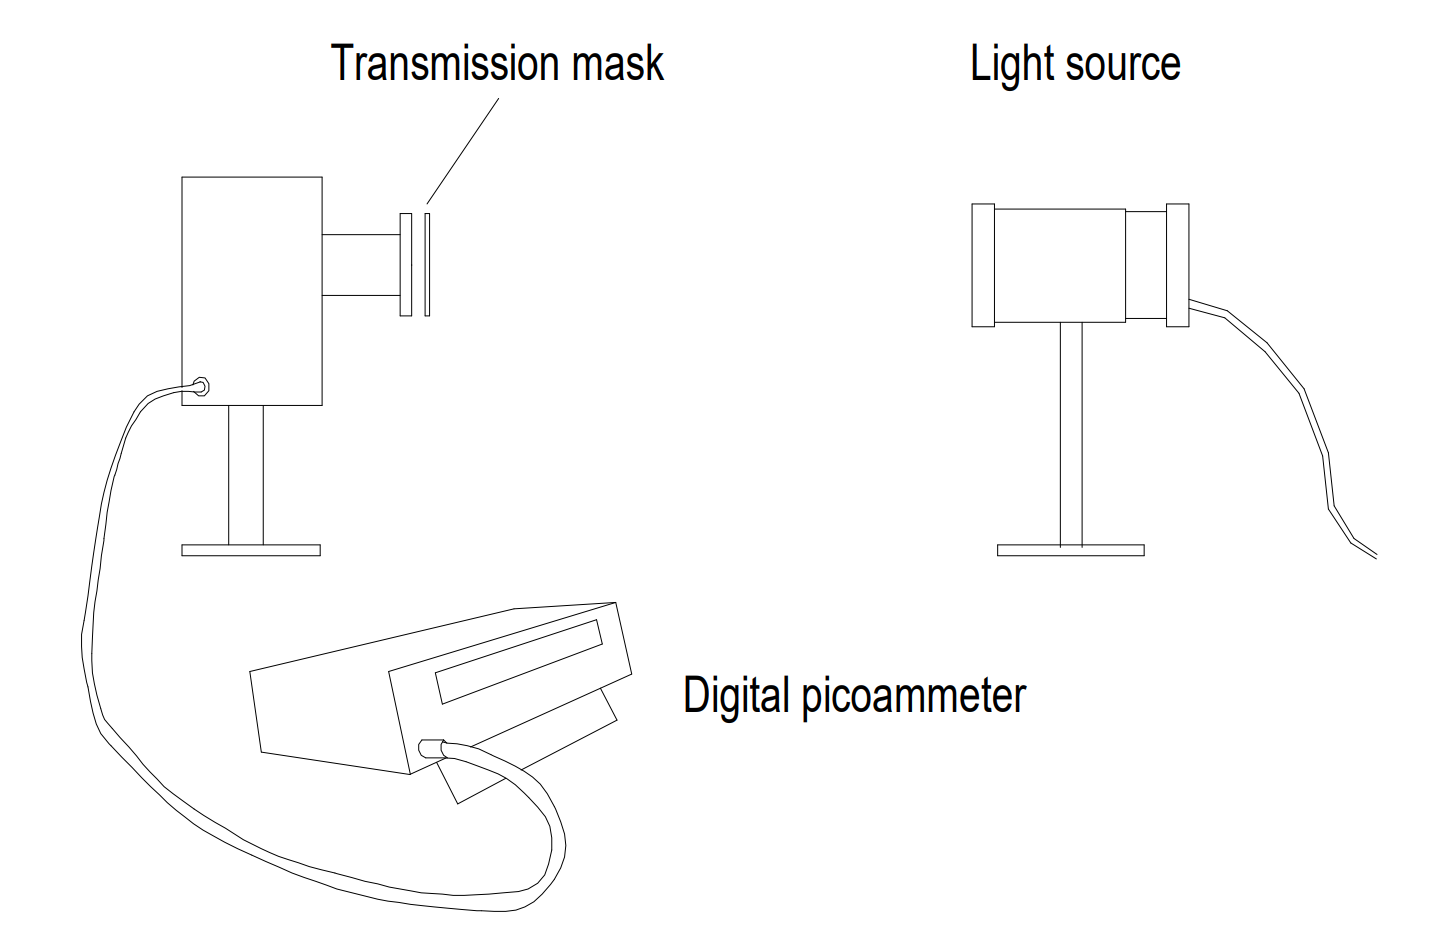
\includegraphics[width=4.08333in,height=2.77083in]{images/06_einstein/001.png}
  \end{center}
\end{figure}

Examine the \emph{variable transmission mask}. This is a strip of
transparent material on which computer-generated patterns of dots and
lines have been printed so as to block selected percentages of the
transparent area and thereby vary the intensity of the transmitted
light. The five sections transmit, respectively, 100\%, 80\%, 60\%,
40\%, and 20\% of the incident light. With the lamp aimed to illuminate
the photocell aperture, hold the transmission mask so that light passes
through the section labeled ``100\%,'' and record the current generated.
Repeat the measurement for the remaining sections and compare the
currents to the corresponding transmission percentages.

\subsection{Electron energy is directly proportional to light frequency.}

It follows from Einstein's equation $\Pi e = h\nu - P$
above that the most energetic electrons among those released from the
illuminated cathode will have kinetic energy \emph{per unit charge} of
amount
\begin{equation*}
\Pi = h\nu/e - P/e
\end{equation*}
where $\nu$~is the frequency of the incident light, \emph{e} is the
charge on the electron, and \emph{P} is a constant characteristic of the
material of the cathode. If \emph{e} is given in abcoulombs and $h$
in erg-seconds, then $\Pi$ will express this energy per unit charge
(the potential) in abvolts. As Einstein states, a
graph of $\Pi$ vs.\ $\nu$ should yield a straight line;
furthermore, it should have a slope equal to \emph{h/e}, having a value
of $4.14\times 10^{-7}$ abvolt/Hz or $4.14\times 10^{-15}$ volt/Hz.\footnote{The
  quotient of presently accepted values $h = 6.625\times 10^{-27}$ erg/Hz
  and $e = 1.6\times 10^{-20}$ abcou is $4.14\times 10^{‑7}$ abvolt/Hz.}

When illuminated, the photocell cathode will lose electrons and thus
acquire a positive potential which continues to increase so long as
electrons continue to flow from it. But, when the cathode potential
rises to a value $\Pi$~that equals the energy per unit charge of the
most energetic electron, no additional electrons will be able to reach
the anode, the photoelectric current will drop to zero, and the
potential will stop rising. An incident light beam will therefore charge
the cathode to the potential $\Pi$; and we can
investigate $\Pi$ as a function of $\nu$ by causing light of
various frequencies to charge the cathode to the corresponding
potentials.

For a source of illumination, we shall use a spectrometer diffraction
grating to separate out individual \emph{spectral lines}\footnote{Glowing
  \emph{gases}, unlike glowing solid bodies, give off light in pure,
  isolated, sharply-demarcated colors, which gives a pattern of isolated
  monochromatic lines separated by wide dark areas when passed through a
  diffraction grating. \emph{Why} this should be is a question which
  Neils Bohr addresses in our next reading: it proves to have a profound
  bearing on atomic structure.} from an intense mercury vapor lamp. The
principal lines are given in the following table:


\begin{minipage}{0.95\textwidth}
\centering
\begin{tabular}{ l l l }
 & $\lambda$ & $\nu$\\
Yellow\footnote{There are really two yellow lines in the mercury
  spectrum, at 5770 and 5882 Å, respectively; but these are not
  separable by the grating and so the line of higher frequency will
  predominate, according to Einstein's treatment.}
  & $5780$ {\small Å}\footnote{One Angstrom (Å) equals $10^{-8}$ cm.}
  & $5.19\times 10^{14}$ Hz\\

Green & $5461$ & $5.49$\\

Blue & $4358$ & $6.88$\\

Violet & $4047$ &$7.41$\\

Ultraviolet & $3655$ & $8.20$\\

\end{tabular}
\end{minipage}

\medskip

Our light source is rich in ultraviolet content and is capable of
damaging the eyes. Suitable protective shielding is provided and you
should not remove it or attempt to defeat its purpose. Needless to say,
\emph{you should avoid looking directly at the beam of light or any
reflections}. Note that the mercury vapor lamp requires a warm-up period
of about five minutes before measurements are made. Also, frequent
on-off operation will reduce the lamp life; once turned on, it is best
to leave it burning until all work for that session is completed.

The apparatus for this part of the experiment is diagrammed here.
\begin{figure}[h]
  \begin{center}
  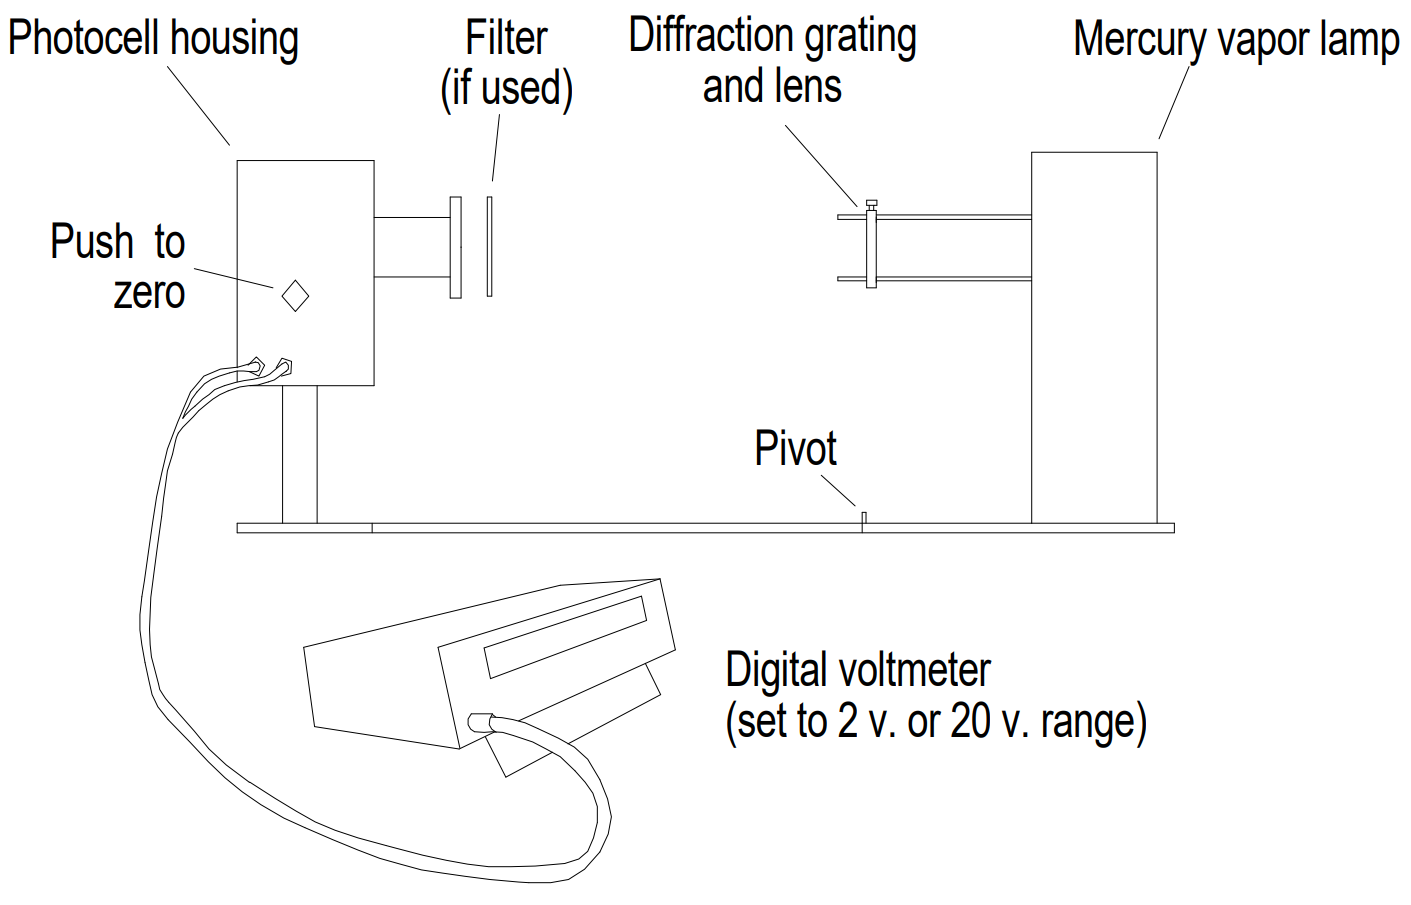
\includegraphics[width=4.08333in,height=2.77083in]{images/06_einstein/003.png}
  \end{center}
\end{figure}


Light exits through a narrow slit at the front of the lamp and is focused on
the photocell aperture by means of an adjustable lens.\footnote{The
  laboratory assistants will have already performed an internal
  alignment to insure that light falling on the aperture fully enters
  the photocell. If you wish to check this adjustment, the procedure is
  described in the final section of this chapter.} A diffraction grating is mounted adjacent to
the lens and forms a spectrum of lines on either side of the beam axis.
The spectrum is significantly brighter on one side than on the other;
make your measurements on the brighter spectrum.

The sketch below shows a top view of the apparatus. Each line of the
Mercury spectrum can be separately introduced to the photocell by moving
the cell to the appropriate position. The spectral lines will be clearly
reflected on the white mask surrounding the photocell aperture. This
mask has been made slightly fluorescent in order to reveal the location
of the otherwise invisible ultraviolet band; it will emit a blue glow
where it is illuminated by ultraviolet light.

\begin{figure}[h]
  \begin{center}
  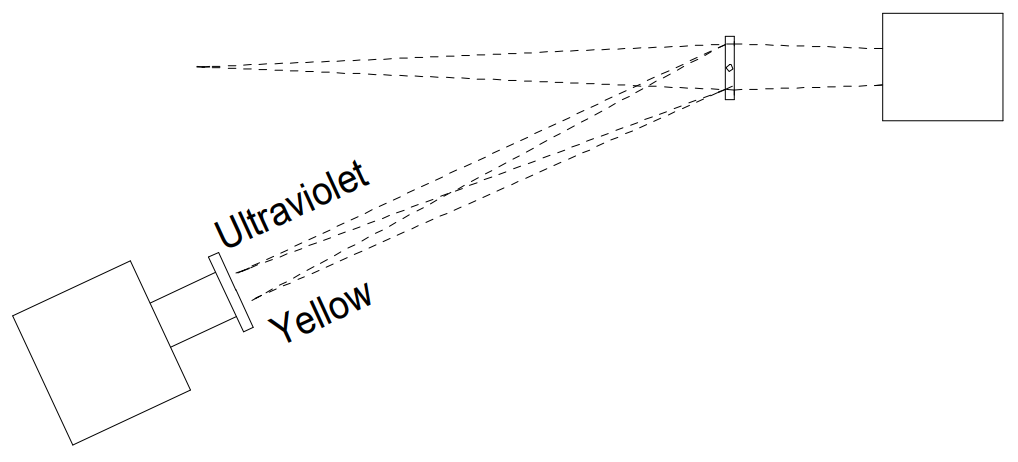
\includegraphics[width=2.91667in,height=1.33333in]{images/06_einstein/005.png}
  \end{center}
\end{figure}


A voltmeter measures the potential difference between the photocell
cathode and anode. But ordinary measuring instruments cannot be
connected to the photocell directly, since they lack sufficient
sensitivity and would actually discharge the photocell in the very
process of measuring its potential. For this part of the experiment,
therefore, the photocell unit is equipped with a battery-powered
amplifier circuit that in effect \emph{reproduces} the cell's potential
difference at a pair of auxiliary terminals. The voltmeter connected to
these terminals will indicate a potential difference equal to that
developed between cathode and anode. Turn the battery switch on at the
beginning of each session, and please remember to turn it off again when
you conclude your work.\footnote{The battery voltage can be tested at
  the two terminals marked ``test.'' Six volts is the minimum acceptable
  reading between each test terminal and the chassis.}

For each measurement, swing the photocell unit until the desired
spectral line falls on the aperture in the cell housing. Take care to
permit only one line at a time to illuminate the aperture. Also, it is
best to confine your measurements to the \emph{first order} of lines
produced by the diffraction grating. Even though the grating will
furnish two or even three orders of spectral lines, the second- and
third-order patterns overlap one another, making some lines unusable.

When measuring the green or yellow spectral lines, be sure to mount the
corresponding green or yellow filter over the face of the cell aperture.
Otherwise ambient light in the room, or even stray reflections from
other spectral lines, might enter the cell housing and cause erroneous
readings. The filters attach easily with magnetic strips. Please treat
the filters with care, as they are easily scratched.

Notice the switch labeled ``push to zero'' on the rear of the photocell
unit. You should operate this switch prior to each reading in order to
discharge any previously accumulated potential difference.

When the photocell is illuminated, and the ``zero'' switch pressed and
released, the voltmeter will gradually rise to a stable value which
represents the maximum potential $\Pi$, corresponding to the
frequency $\nu$ of the light presently being admitted to the
cell.\footnote{In some devices, the voltmeter will temporarily read
  \emph{high} and gradually \emph{decrease} to a stable value. This
  reflects a variation in the manufacturer's amplifier circuit; but the
  stable reading nevertheless indicates the actual potential difference
  in the photocell.}

Our digital voltmeters perform poorly when their batteries run down;
\emph{please} turn off the voltmeters at the end of each session. If the
readings obtained for bright spectral lines appear to be erratic, try
another voltmeter, or replace the battery. But note that when the
photocell is \emph{not} illuminated, it is normal for the voltmeter
readings to drift randomly.

\subsubsection*{INTERNAL ALIGNMENT --- Adjust only if necessary}

\begin{tight_enumerate}
\item Swing the photocell to the side having the brighter diffraction
pattern until the green line, say, falls on the white mask surrounding
the photocell aperture.

\item Roll the cylindrical light shield out of the way to reveal a second
white mask with a smaller aperture. Loosen the thumbscrew on the
photocell housing support rod and rotate the photocell unit until the
green line is centered both on the aperture of the external mask
\emph{and} the aperture of the internal mask, simultaneously. Tighten
the support rod thumbscrew securely.

\item Loosen the thumbscrew on the diffraction grating/lens assembly and
slide it back and forth on the support rods to focus the light onto the
internal white mask. Roll the cylindrical light shield back into
position; tighten the grating/lens thumbscrew to hold the assembly in
place.

\item For additional alignment accuracy, repeat steps 2 and 3 again.
\end{tight_enumerate}
